\section{Metagenome}

\subsection{\textit{Musca domestica} salivary gland hypertrophy virus}
\begin{frame}
Assembly: 124,552 bp, 100 CDS (96 identified as the reference)\\
DNA polymerase (identities: 966/979 (99\%), gaps: 3/979 (0\%))\\
% {\scriptsize
% {\ttfamily
% Query  1    MLLRPNYQYNWSDDDDDDN-SVCESEQSYRSRSPSPLPWTSSSSTVTCMISDIKTQAYAN  59
%             MLLRPNYQYNWSDDDDDD+ +  ESEQSYRSRSPSPLPWTSSSSTVTCMISDIKTQAYAN
% Sbjct  1    MLLRPNYQYNWSDDDDDDSVNDNESEQSYRSRSPSPLPWTSSSSTVTCMISDIKTQAYAN  60
% Query  60   RVVNIKLSLMNEYGEKLLKLIQGDVFFDVYIETWNRNENIARILNQLQCYNNTPQFVDTK  119
%             RVVNIKLSLMNEYGEKLLKLIQGDVFFDVYIETWNRNENIARILNQLQCYNNTPQFVDTK
% Sbjct  61   RVVNIKLSLMNEYGEKLLKLIQGDVFFDVYIETWNRNENIARILNQLQCYNNTPQFVDTK  120
% Query  120  YTAMGYSQTPLNVWRLNIRENRLDYIYEFCQSSGRRMFLNTELNDALPMVQKNLGIYCDI  179
%             YTAMGYSQTPLNVWRLNIRENRLDYIYEFCQSSGRRMFLNTELNDALPMVQKNLGIYCDI
% Sbjct  121  YTAMGYSQTPLNVWRLNIRENRLDYIYEFCQSSGRRMFLNTELNDALPMVQKNLGIYCDI  180
% Query  180  PNVGDTAQIPYSSLTKPDMSTPKSFICRKLSIDIEVITPPEWTLFPDATELGCEIIIIAC  239
%             PNVGDTAQIPYSSLTKPDMSTPKSFICRKLSIDIEVITPPEWTLFPDATELGCEIIIIAC
% Sbjct  181  PNVGDTAQIPYSSLTKPDMSTPKSFICRKLSIDIEVITPPEWTLFPDATELGCEIIIIAC  240
% Query  240  TRQQDDTTTYQTDILYTDSQHREIRIENADNRNFIRFDTEYQMLEYFITSIDPHNTDLLT  299
%             TRQQDDTTTYQTDILYTDSQHREI IENADNRNFIRFDTEYQMLEYFITSIDPHNTDLLT
% Sbjct  241  TRQQDDTTTYQTDILYTDSQHREIHIENADNRNFIRFDTEYQMLEYFITSIDPHNTDLLT  300
% Query  300  GWNVRNFDLKYIYDRCCKFFPDLVAKFRQWTLDGSDISFRNVTRKGQNVTLVESFGIMIL  359
%             GWNVRNFDLKYIYDRCCKFFPDLVAKFRQWTLDGSDISFRNVTRKGQNVTLVESFGIMIL
% Sbjct  301  GWNVRNFDLKYIYDRCCKFFPDLVAKFRQWTLDGSDISFRNVTRKGQNVTLVESFGIMIL  360
% Query  360  DMYDYNKSNVKAKSYKLKDIARKYLREDKQKLDIDYKDISRFYRSGNTKEFSHLLEYCSV  419
%             DMYDYNKSNVKAKSYKLKDIARKYLREDKQKLDIDYKDISRFYRSGNTKEFSHLLEYCSV
% Sbjct  361  DMYDYNKSNVKAKSYKLKDIARKYLREDKQKLDIDYKDISRFYRSGNTKEFSHLLEYCSV  420
% Query  420  DAEIVLDLMAVQKVWNNTVSMADICHVPMNYVVNSGVMLRNTCMISQFVNEHTDYLLPYK  479
%             DAEIVLDLMAVQKVWNNTVSMADICHVPMNYVVNSGVMLRNTCMISQFVNEHTDYLLPYK
% Sbjct  421  DAEIVLDLMAVQKVWNNTVSMADICHVPMNYVVNSGVMLRNTCMISQFVNEHTDYLLPYK  480
% Query  480  HEMPFTSYEGGYVNEPIVGFHTDPIFVLDFNSLYPTTMLAFNICTTTIVDMREYSDTGYP  539
%             HEMPFTSYEGGYVNEPIVGFHTDPIFVLDFNSLYPTTMLAFNICTTTIVDMREYSDTGYP
% Sbjct  481  HEMPFTSYEGGYVNEPIVGFHTDPIFVLDFNSLYPTTMLAFNICTTTIVDMREYSDTGYP  540
% Query  540  IDAIPSTSSSSDTTPYQPTELDQVVFTTSNELKISATPYMHNVGFVAANHRRGVMPQILH  599
%             IDA+PST  SSDTTPYQPTELDQV+FTTSNELKISATPYMHNVGFVAANHRRGVMPQILH
% Sbjct  541  IDAMPST--SSDTTPYQPTELDQVIFTTSNELKISATPYMHNVGFVAANHRRGVMPQILH  598
% Query  600  NLLTTRKRLQNELKKTTDDQKRKQLDAQQLSYKLCANAIYGLLGCSFSPLYNPMVAASVT  659
%             NLLTTRKRLQNELKKTTDDQKRKQLDAQQLSYKLCANAIYGLLGCSFSPLYNPMVAASVT
% Sbjct  599  NLLTTRKRLQNELKKTTDDQKRKQLDAQQLSYKLCANAIYGLLGCSFSPLYNPMVAASVT  658
% Query  660  SFGRFLSYIKRKRITEYMAAENIEGSIVYGDTDSVMVQIRNHTIAETKAIAERYAEQVTR  719
%             SFGRFLSYIKRKRITEYMAAENIEGSIVYGDTDSVMVQIRNHTIAETKAIAERYAEQVTR
% Sbjct  659  SFGRFLSYIKRKRITEYMAAENIEGSIVYGDTDSVMVQIRNHTIAETKAIAERYAEQVTR  718
% Query  720  DIGIPPIRTEYEKIFCPFLIHKKKHYIGVMYTDNCDRHLRVEYKGNEMVRSDNCTLTTDV  779
%             DIGIPPIRTEYEKIFCPFLIHKKKHYIGVMYTDNCDRHLRVEYKGNEMVRSDNCTLTTDV
% Sbjct  719  DIGIPPIRTEYEKIFCPFLIHKKKHYIGVMYTDNCDRHLRVEYKGNEMVRSDNCTLTTDV  778
% Query  780  MRDVIDLLFFGDGDLTQKNAAITRRLEELLAEWSQLYGMYREGTPVDRELRTRVVQQAIY  839
%             MRDVIDLLFFGDGDLTQKNAAITRRLEELLAEWSQLY MYREGTPVDRELR RVVQQAIY
% Sbjct  779  MRDVIDLLFFGDGDLTQKNAAITRRLEELLAEWSQLYNMYREGTPVDRELRARVVQQAIY  838
% Query  840  SKKLAKEVYTNRLPHVAVYERMKNRKQYHIGDRIVYCIANTELSDRVKPKNIIDMAYDID  899
%             SKKLAKEVYTNRLPHVAVYERMKNRKQYHIGDRIVYCIANTELSDRVKPKNIIDMAYDID
% Sbjct  839  SKKLAKEVYTNRLPHVAVYERMKNRKQYHIGDRIVYCIANTELSDRVKPKNIIDMAYDID  898
% Query  900  EFLEDERLYLAVHYYADACVRKPLSRLFASLDSQFRTQLELTLSRLFPSLVASAQKRAHK  959
%             EFLEDE+LYLAVHYYADACVRKPLSRLFASLDSQFRTQLELTLSRLFPSLVASAQKRAHK
% Sbjct  899  EFLEDEQLYLAVHYYADACVRKPLSRLFASLDSQFRTQLELTLSRLFPSLVASAQKRAHK  958
% Query  960  DKETAVLCKQKKSCENKRQ  978
%             DKETAVLCKQKKSCENKRQ
% Sbjct  959  DKETAVLCKQKKSCENKRQ  977
% }
% }
\begin{center}
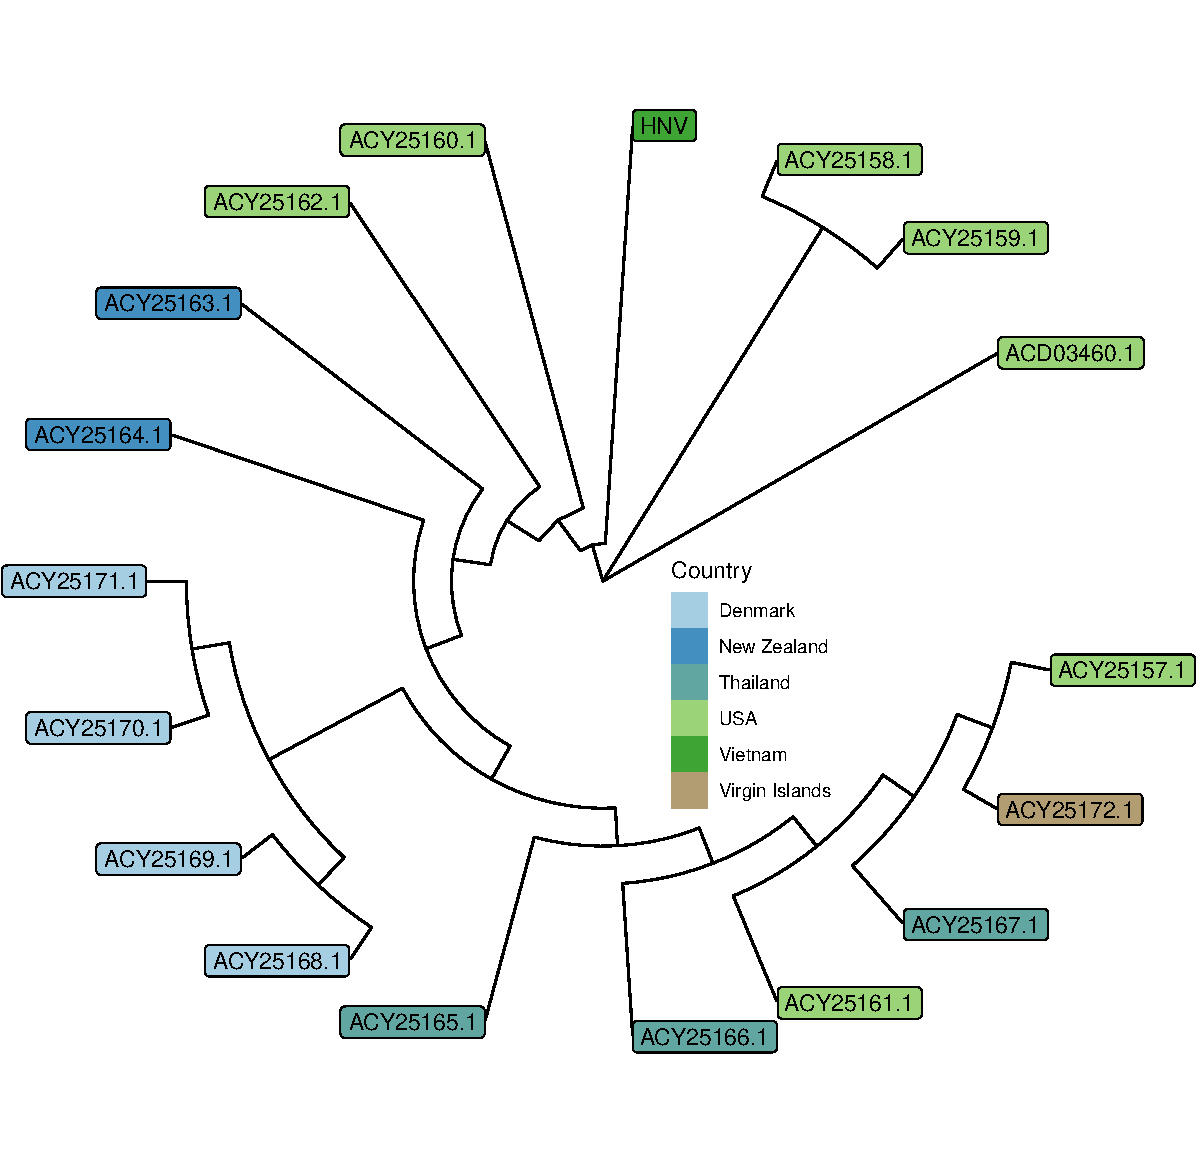
\includegraphics[trim=0cm 1.8cm 0cm 1.8cm, clip, width=0.7\textwidth]{../Viet_seq/fig_phylob.pdf}
\end{center}
\footnotetext{HNV.07, 5 NAGY secret egész}
\end{frame}

\subsection{\textit{Haematobia irritans} densovirus}
\begin{frame}
Assembly: 4,841 bp (depth 520)\\

\begin{center}
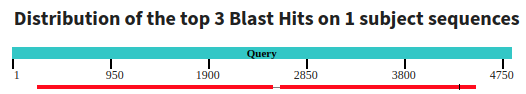
\includegraphics[width=0.8\textwidth]{../Viet_seq/HIdensovirus.png}
\end{center}

\textit{Haematobia irritans} densovirus isolate HiDV/URU, partial genome\\
4,283 bp\\
Uruguay\\
Range 1: 43 to 2329, identities: 2112/2290(92\%), gaps: 8/2290(0\%)\\
Range 2: 2326 to 4056, identities: 1517/1734(87\%), gaps: 6/1734(0\%)\\
Range 3: 4109 to 4280, identities: 156/172(91\%), gaps: 1/172(0\%)\\
\footnotetext{45-NAGY-M, 5 nagy vérszívó}
\end{frame}

\subsection{Pathogens}
\begin{frame}

\begin{center}
{\tiny%
\begin{tabular}{llrlrr}
\toprule
Sample & Contig & bp & Best match & Identities & Gaps \\
\midrule
TNV\_09 & k59\_7 & 239 & Anaplasma marginale strain Jaboticabal & 239/239 (100\%) & 0/239 (0\%)\\
 & k59\_30 & 255 & Anaplasma marginale strain Jaboticabal & 255/255 (100\%) & 0/255 (0\%)\\
HNV\_07 & k141\_5 & 307 & Trypanosoma vivax Y486 & 84/97 (87\%) & 7/97 (7\%)\\
 & k141\_10 & 349 & Leishmania amazonensis strain UA301 & 131/133 (98\%) & 0/133 (0\%)\\
 & k141\_1 & 324 & Leishmania donovani strain LdCL & 257/306 (84\%) & 2/306 (0\%)\\
 & k141\_7 & 512 & Leishmania donovani strain LdCL & 385/456 (84\%) & 0/456 (0\%)\\
 & k141\_22 & 369 &  Trypanosoma vivax Y486 & 355/369 (96\%)  & 0/369 (0\%)\\
 & k141\_4 &  397& Leishmania donovani strain Dd8 & 321/382 (84\%) & 14/382 (3\%)\\
 & k141\_14 & 742 & Trypanosomatidae sp. GMO-05 & 580/581 (99\%) & 0/581 (0\%) \\
 & k141\_18 & 1079 & Trypanosoma kuseli & 749/825 (91\%) & 19/825 (2\%)\\
 & k141\_19 & 1168 & Trypanosoma theileri YMG-11 & 1033/1141 (91\%) & 42/1141 (3\%)\\
 & k141\_20 & 1662 & Leptomonas pyrrhocoris & 1519/1666 (91\%) & 5/1666 (0\%)\\
 & k141\_21 & 3062 & Trypanosomatidae sp. GMO-05 & 1114/1120 (99\%) & 1/1120 (0\%)\\
\bottomrule
\end{tabular}
}
\end{center}
\end{frame}

% TNV_09_S2022_NAGY-M_anaplasma_final.contigs.fa
% k59_7 flag=1 multi=2.0000 len=239
% Anaplasma marginale strain Jaboticabal chromosome
% 239/239(100%)	0/239(0%)
%
% k59_30 flag=1 multi=2.0000 len=255
% Anaplasma marginale strain Jaboticabal chromosome
% 255/255(100%)	0/255(0%)
%
% HNV_07_S2022_NAGY_M_trypanosoma_final.contigs.fa
% k141_5 flag=1 multi=4.0000 len=307
% Trypanosoma vivax Y486 annotated genomic contig, chromosome 11
% 84/97(87%)	7/97(7%)
%
% k141_10 flag=1 multi=4.0000 len=349
% Leishmania amazonensis strain UA301 chromosome 27
% 131/133(98%)	0/133(0%)
%
% 141_1 flag=1 multi=4.0000 len=324
% Leishmania donovani strain LdCL chromosome LdCL_35, complete sequence
% 257/306(84%)	2/306(0%)
%
% k141_7 flag=1 multi=3.0000 len=512
% Leishmania donovani strain LdCL chromosome LdCL_15, complete sequence
% 385/456(84%)	0/456(0%)
%
% k141_22 flag=3 multi=3.0132 len=369
% Trypanosoma vivax Y486 annotated genomic contig, chromosome 11
% 355/369(96%)	0/369(0%)
%
% k141_4 flag=1 multi=3.0000 len=397
% Leishmania donovani strain Dd8 histone H3 gene, partial cds
% 321/382(84%)	14/382(3%)
%
% k141_14 flag=1 multi=6.0000 len=742
% Trypanosomatidae sp. GMO-05 small subunit ribosomal RNA gene, partial sequence
% 580/581(99%)	0/581(0%)
%
% k141_18 flag=1 multi=4.0000 len=1079
% Trypanosoma kuseli genes for IGS, 18S rRNA, 5.8S rRNA, 28S rRNA and ITS1-6
% 749/825(91%)	19/825(2%)
%
% k141_19 flag=1 multi=3.0000 len=1168
% Trypanosoma theileri YMG-11 genes for 18S rRNA, ITS1, 5.8S rRNA, ITS2, 28S rRNA, ITS3, ITS4, ITS5, partial and complete
% sequence
% 1033/1141(91%)	42/1141(3%)
%
% k141_20 flag=1 multi=6.0000 len=1662
% Leptomonas pyrrhocoris putative mitochondrial heat-shock protein hsp70 mRNA
% 1519/1666(91%)	5/1666(0%)
%
% k141_21 flag=1 multi=5.0000 len=3062
% Trypanosomatidae sp. GMO-05 small subunit ribosomal RNA gene, partial sequence
% 1114/1120(99%)	1/1120(0%)



%
% 32-NAGY-M
% 5 nagy vérszívó

% 33-NAGY-M
% 5 nagy vérszívó
%
% 34-KICSI-M
% 4 kicsi vérszívó
%
% 35-NAGY-M
% 4 nagy vérszívó
%
% 37-NAGY-M
% 1 nagy vérszívó
%
% 38-NAGY-M
% 1 nagy vérszívó
%
% 39-NAGY-M
% 1 nagy vérszívó
%
% 40-NAGY-M
% 4 nagy vérszívó
%
% 41-KICSI-M
% 4 nagy  vérszívó
%
% 41-NAGY-M
% 4 kicsi vérszívó
%
% 42-NAGY-M
% 5 nagy szekretofág
%
% 43-NAGY-M
% 5 nagy vérszívó
%
% 45-NAGY-M
% 5 nagy vérszívó
%
% 59-NAGY-M
% 5 nagy vérszívó
%
% TNV.05.S2022
% 3 NAGY secret egész
%
% körTNV.06.S2022
% 3 NAGY vérszívó egész
%
% TNV.09.S2022
% 3 NAGY vérszívó egész
%
% HNV.07.S2022
% 5 NAGY secret egész
%
% TBV.22. S 2022
% 3 KICSI egész + 1 nagy

